\documentclass[11pt]{article}

%Format and referencing 
\usepackage[letterpaper,top=2cm,bottom=2cm,left=1.5cm,right=2cm,marginparwidth=1.75cm]{geometry} % for setting margins VERY IMPORTANT!
\usepackage{hyperref}  % for referencing equations 
\usepackage{biblatex}  % for referencing articles 
\addbibresource{Bib.bib}


%math packages 
\usepackage{mathtools}  % allows pre-scripts and other neiche math features
\usepackage{amsmath} % equation related commands 
\usepackage{amssymb} % Fancy R ,C and other set fonts using mathbb{}
\usepackage{braket}   % for Dirac notation 
\usepackage{mathrsfs}  % for the mathscr text 
\usepackage{bbm} % for identity matrix

% miscellaneous
\usepackage{empheq}   % for formatting custon math boxs
\usepackage{xcolor}   % allows the defining of colours 
\usepackage[most]{tcolorbox}  % custom math boxs
\usepackage[utf8]{inputenc}   % redundant since 2018? 
%(I'm not taking out in case it breaks stuff)

\usepackage{graphicx}   % alows image insertion 
\usepackage{float}  % for making images o where you want 
\usepackage{parskip} % for getting red of paragraph indent 

\usepackage{comment} %easier multi line comments 
 \usepackage{tabularx} % for formatting tables 
 \usepackage{titling} % for making Title a variable that can be used in header 
 \usepackage{environ} % for creating and modifying environments 
 \usepackage[explicit]{titlesec}
 % for making section titles variables that can be used in header 
\usepackage{fancyhdr} % for fancy headers 

% Random commands and what not 
\numberwithin{equation}{section}

\setlength{\droptitle}{3em} 

{\Huge  
\title{Standard Model}
\author{Thomas Brosnan}
\date{Notes taken in Professor Ruth Britto's class, Hillary term 2025}
}

\DeclarePairedDelimiterXPP\BigOSI[2]%
  {\mathcal{O}}{(}{)}{}%
  {\SI{#1}{#2}}

\newtcbox{\mymath}[1][]{%
    nobeforeafter, math upper, tcbox raise base,
    enhanced, colframe=blue!30!black,
    colback=blue!30, boxrule=1pt,
    #1}
\tcbset{highlight math style={boxsep=2mm,,colback=blue!0!green!0!red!0!}}

\newenvironment{bux}{\empheq[box=\tcbhighmath]{align}}{\endempheq}
\newenvironment{bux*}{\empheq[box=\tcbhighmath]{align*}}{\endempheq}
\renewenvironment{flalign}{\vspace{-3mm}\empheq[box=\tcbhighmath]{align}}{\endempheq}
\renewenvironment{flalign*}{\vspace{-3mm}\empheq[box=\tcbhighmath]{align*}}{\endempheq}
%\renewenvironment{align}{\vspace{-5mm}\begin{align}}{\end{align}}
%\renewenvironment{align*}{\vspace{-5mm}\begin{align*}}{\end{align*}}
\renewenvironment{alignat}{\empheq{align*}}{\endempheq}


\newcommand{\hsp}{\hspace{8pt}}

\newcommand{\I}[1]{\emph{#1}}

\newcommand*{\sectionFont}{%
  \LARGE\bfseries
}

\newenvironment{eq}{\begin{equation}}{\end{equation}}
    


\makeatletter
\let\Title\@title % Copy the title to a new command
\makeatother

%change this RGB value to change the section background colour 
\definecolor{mycolor1}{RGB}{252,149,183}
\colorlet{SectionColour}{mycolor1}
%subsection background colour 
\definecolor{mycolor2}{gray}{0.8}
\colorlet{subSectionColour}{mycolor2}
%subsubsection background colour 
\definecolor{mycolor3}{RGB}{255,255,255}
\colorlet{subsubSectionColour}{mycolor3}



\begin{document}

\maketitle

\newpage
\topskip0pt
\vspace*{\fill}
\begin{center}
\Large
    "If you can't explain it simply enough you don't understand it well enough"
    
    - Albert Einstein
\end{center}
\vspace*{\fill}
\newpage 
\tableofcontents
% For \section
 \titleformat{\section}[block]{\sectionFont}{}{0pt}{%
 \fcolorbox{black}{SectionColour}{\noindent\begin{minipage}{\dimexpr\textwidth-2\fboxsep-2\fboxrule\relax}\thesection  \hsp #1 {\strut} \end{minipage}}}
% For \subsection
 \titleformat{\subsection}[block]{\bfseries}{}{0pt}{%
 \fcolorbox{black}{subSectionColour}{\noindent\begin{minipage}{\dimexpr\textwidth-2\fboxsep-2\fboxrule\relax}\thesubsection  \hsp #1 {\strut} \end{minipage}}}
% For \section*
 \titleformat{name=\section, numberless}[block]{\sectionFont}{}{0pt}{%
 \fcolorbox{black}{SectionColour}{\noindent\begin{minipage}{\dimexpr\textwidth-2\fboxsep-2\fboxrule\relax} #1 {\strut} \end{minipage}}}
  % For \subsection*
 \titleformat{name=\subsection, numberless}[block]{\bfseries}{}{0pt}{%
 \fcolorbox{black}{subSectionColour}{\noindent\begin{minipage}{\dimexpr\textwidth-2\fboxsep-2\fboxrule\relax} #1 {\strut} \end{minipage}}}
 % For \subsubsection
 \titleformat{\subsubsection}[block]{\bfseries}{}{0pt}{%
 \fcolorbox{black}{subsubSectionColour}{\noindent\begin{minipage}{15cm}\thesubsubsection \hsp #1 {\strut} \end{minipage}}}
  % For \subsubsection*
 \titleformat{name=\subsubsection, numberless}[block]{\bfseries}{}{0pt}{%
 \fcolorbox{black}{subsubSectionColour}{\noindent\begin{minipage}{15cm} #1 {\strut} \end{minipage}}}
\newpage 
%header and footer
\pagestyle{fancy}
\fancyhf{} % Clear all header and footer fields
\fancyhead[L]{\Title}
\fancyhead[R]{\nouppercase{\leftmark}}
\fancyfoot[C]{-~\thepage~-}
\renewcommand{\headrulewidth}{1pt}




%starting document 
\normalsize
\newpage
\section{The Quark Model}
\begin{itemize}
    \item Long ago it was realized that the proton and the neutron have very similar masses and thus in regions where the Electromagnetic is weak compared to the strong force, there is an approximate symmetry between the neutron. With this, it was postulated that these two particles were two states of the same particle, \emph{the nucleon}. With this in analogous to spin states, we can write the proton as $\ket{p} = (1,0)^T$ and the neutron as $\ket{n} = (0,1)^T$. This lead to the idea of \emph{Isospin}, as the proton and the neutron can be considered to form an isospin doublet, with total Isospin $1/2$ and a third component of $I_3 = \pm1/2$. Just like spin, our Lagrangian (if we ignore the electromagnetic terms) should be invariant under unitary transformations of these states (which will be $\in U(2)$), meaning there is a conserved charge associate with this transformation. We can do this exact same procedure for the up and down quarks. The strong force treats all the quarks equally, and seeing as the up and down quark have approximately the same masses, we can treat them as spin states just like the nucleon. In this case the conserved quantity associated with this symmetry is known as \emph{flavor}. 
\end{itemize}

\subsection{Isospin} % (fold)
\label{sub:isospin}
\begin{itemize}
    \item  $U(2)$ has $4$ degrees of freedom, and thus $4$ generators, one of these can be chosen to be a scaling by a phase factor of the identity, $e^{i\theta}\mathbbm{1}$, since overall phase factors of $U(1)$ do not change our states, this can be ignored, leaving us with the $3$ Pauli matrices $\sigma^i$, which are the generators of $SU(2)$, the main symmetry group here. From this we can proceed in the exact same manner as we do with spin, recognizing that these matrices form a non-Abelian Lie algebra based on their commutators, where we can define raising and lowering operators, to enable us to write down states analogous to $\ket{lm}$ for spin. This quantity that is like spin is called \emph{Isospin}. This is 3-vector and is defined as:
    \begin{align*}
        \textbf{T} = \frac{1}{2}\boldsymbol{\sigma}
    \end{align*}
    \item The components obey the following commutations relations:
    \begin{align*}
         [T_i,T_j] = i\epsilon_{ijk}T_k
     \end{align*} 
     Where we have sum of the index $k$. The measurable quantity from this system is the total isospin, $ \textbf{T}^2 = T_1^2+T_2^2+T_3^2$. We will label states by their total isospin and the third component of isospin $I_3$, i.e. $\phi(I,I_3)$. The up quark is then $\ket{u} = \phi(\frac{1}{2},\frac{1}{2})$ and the down quark is $\ket{d} = \phi(\frac{1}{2},-\frac{1}{2})$. 
\end{itemize}
% subsection isospin (end)

\subsection{Anti-quark Doublet} % (fold)
\label{sub:anti_quark_doublet}
\begin{itemize}
    \item The above treatment of up and down quarks is called a \emph{quark doublet}, which we write as:
    \begin{align*}
        q = \left(\begin{matrix}
            u \\ d
        \end{matrix}\right)
    \end{align*}
We would like to have the same treatment of anti-quarks. We know that the complex conjugate of any quark will give us the anti-quark (eg. $u^{\ast} = \bar{u}$), but we don't want to write down something like $\bar{q} = (\bar{u},\bar{d})^{T}$ as then this will transform via $U^{\ast}$ instead of $U$ and will not follow the same symmetries. Instead we should find some combination that does transform via $U$. We write this as $\bar{q} = S(\bar{u},\bar{d})^{T}$ and then impose that $SU^{\ast} = US$. Solving this equation results in the matrix $S= \begin{pmatrix}
    0 & -1 \\ 1 & 0 
\end{pmatrix}$. Meaning the quark anti-state can be written as:
\begin{align*}
    \bar{q} = \begin{pmatrix}
        -\bar{d} \\ \bar{u}
    \end{pmatrix}
\end{align*}

\end{itemize}
% subsection anti_quark_doublet (end)

\subsection{Mesons} % (fold)
\label{sub:mesons}
\begin{itemize}
    \item Mesons are bound states of a quark and anti-quark pair, since quarks are spin half, this makes mesons bosons. Since Mesons are comprised of two quarks, we can think of adding their Isospin in exactly the same way we add the spin of two particles together. Since the quarks have isospin $\frac{1}{2}$, this will create the familiar $\frac{1}{2} \otimes \frac{1}{2} = 1 \oplus 0$. Meaning there will be four possible states, a triplet with $I_3=1$ and a singlet with $I_3=0$. These state correspond to meson particles! Each state will correspond to more then one particle as we are not considering different combinations of spins (which affect the mass!). These particles are:
\begin{align*}
    &\phi(1,1) = -|\! u\bar{d} \rangle \; &=& |\pi^{+} \rangle, |\rho^{+} \rangle \\ 
    &\phi(1,0) = \frac{1}{\sqrt{2}}\left(|\! u\bar{u} \rangle - |\! d\bar{d} \rangle \right) \; &=& |\pi^{0} \rangle, |\rho^{0} \rangle \\ 
    &\phi(1,-1) = |\! d\bar{u} \rangle \; &=& |\pi^{-} \rangle, |\rho^{-} \rangle \\ 
    &\phi(0,0) = \frac{1}{\sqrt{2}}\left(|\! u\bar{u} \rangle + |\! d\bar{d} \rangle \right) \; &=& |\eta \rangle, |\omega \rangle
\end{align*}

\end{itemize}
% subsection mesons (end)

\subsection{$SU(3)$ Flavour} % (fold)
\label{sub:su3}
\begin{itemize}
    \item The above described $SU(2)$ symmetry is almost exact as the up and down quarks have almost them same mass. What we can also do is consider extending this symmetry to the strange quark. This makes it a $SU(3)$ symmetry, as the quark doublet now becomes a quark triplet $q= (u,d,s)^T$, for which we will need a new basis of generators. The standard choice of generators are the \emph{Gell Mann matrices}:
\begin{align*}
    \lambda_1 &= \begin{pmatrix} 0 & 1 & 0 \\ 1 & 0 & 0 \\ 0 & 0 & 0 \end{pmatrix}, &
    \lambda_2 &= \begin{pmatrix} 0 & -i & 0 \\ i & 0 & 0 \\ 0 & 0 & 0 \end{pmatrix}, &
    \lambda_3 &= \begin{pmatrix} 1 & 0 & 0 \\ 0 & -1 & 0 \\ 0 & 0 & 0 \end{pmatrix},~~~ u \leftrightarrow d \\[10pt]
    %
    \lambda_4 &= \begin{pmatrix} 0 & 0 & 1 \\ 0 & 0 & 0 \\ 1 & 0 & 0 \end{pmatrix}, &
    \lambda_5 &= \begin{pmatrix} 0 & 0 & -i \\ 0 & 0 & 0 \\ i & 0 & 0 \end{pmatrix}, &
    & u \leftrightarrow s \\[10pt]
    %
    \lambda_6 &= \begin{pmatrix} 0 & 0 & 0 \\ 0 & 0 & 1 \\ 0 & 1 & 0 \end{pmatrix}, &
    \lambda_7 &= \begin{pmatrix} 0 & 0 & 0 \\ 0 & 0 & -i \\ 0 & i & 0 \end{pmatrix}, &
    & d \leftrightarrow s \\[10pt]
    %
    \lambda_8 &= \frac{1}{\sqrt{3}} \begin{pmatrix} 1 & 0 & 0 \\ 0 & 1 & 0 \\ 0 & 0 & -2 \end{pmatrix},~~~&&\text{equal treatment of u,d}
\end{align*}
\item This particular choice is normalized such that $\text{tr}(\lambda_i\lambda_j) = 2\delta_{ij}$. With this we can define the $SU(3)$ Isospin in a similar manner to $SU(2)$ by identifying:
\begin{align*}
     \hat{T}_i = \frac{1}{2}\lambda_i
 \end{align*} 
 The total Isospin is then $\sum_i T^2_i = \frac{1}{4}\lambda_i^2 = \frac{4}{3}\mathbbm{1}$. $SU(3)$ is different to $SU(2)$ in the fact that it two mutually commuting generators instead of $1$. We can call once again the component along the direction of the third generator $T_3$ the third component of the isospin $I_3$ and identify states by this number, but we then also need to consider the component along the direction of $\hat{T}_8$ as $\hat{T}_8$ commutes with $\hat{T}_3$. The component along this direction is known as the \emph{Hyper-charge} and is denoted with a $Y$. Strictly we define the hyper charge to be $Y = \frac{1}{\sqrt{3}}\lambda_8$. 

 \item From the definitions of the Gell Mann matrices we can check the values of the $I_3$ and $Y$, for the 3 quarks:
\begin{align*}
    \hat{T}_3 u &= +\frac{1}{2} u & \quad \hat{Y} u &= +\frac{1}{3} u \\
    \hat{T}_3 d &= -\frac{1}{2} d & \quad \hat{Y} d &= +\frac{1}{3} d \\
    \hat{T}_3 s &= 0 & \quad \hat{Y} s &= -\frac{2}{3} s
\end{align*} 

 We can plot $Y$ and $I_3$ for the three quarks and their anti-particles:
 \begin{figure}[H]
\centering
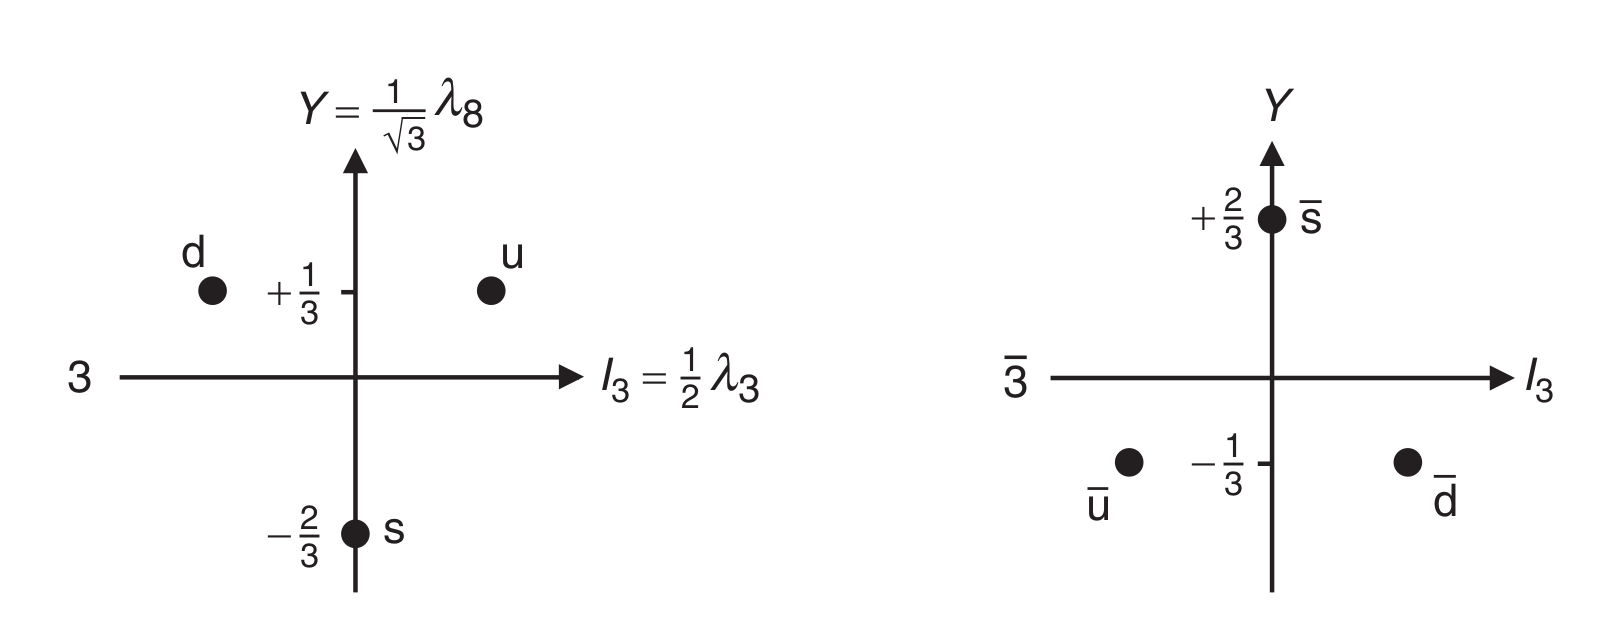
\includegraphics[width=0.6\textwidth]{Hypercharge.png}
\caption{\label{trailer}\emph{Quark Isospin and Hyper-charge}}
\end{figure}  
\end{itemize}
% subsection su3 (end)

\subsection{Light Mesons} % (fold)
\label{sub:light_mesons}
\begin{itemize}
\item Since we have used $\lambda_3$ and $\lambda_8$ to form what is know as the Cartan sub-algebra, we can take the remaining $\lambda_i$ and form raising and lowering operators. There will be three pairs, that which step respectively between the $d \leftrightarrow u, s\leftrightarrow u$ and $d\leftrightarrow s$:
\begin{align}
    \hat{T}_\pm &= \frac{1}{2} (\lambda_1 \pm i \lambda_2) \\
    \hat{V}_\pm &= \frac{1}{2} (\lambda_4 \pm i \lambda_5) \\
    \hat{U}_\pm &= \frac{1}{2} (\lambda_6 \pm i \lambda_7)
\end{align}
We can use these to find all possible Mesons made out of these $3$ quarks. This is done by identifying the extreme states (stats with maximal $I_3$ or $Y$), then apply the raising and lowering operators to exhaust all other possible states. Since we are combining $3$ possible quarks with $3$ possible anti-quarks \footnote{Here we are only looking at 2 quark combinations here, i.e. Mesons} then this is a case of $3 \otimes \bar{3} = 8 \oplus 1$ \footnote{The bar on the $3$ just indicates that this is the anti-quark triplet}. This decomposition is into a octet and a singlet and takes the below visual form:
 \begin{figure}[H]
\centering
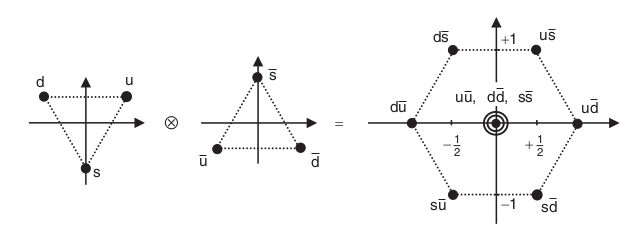
\includegraphics[width=0.5\textwidth]{3x3}
\caption{\label{trailer}\emph{Decomposition of quark-anti-quark combinations }}
\end{figure} 
Where the singlet is plotted along with the two octet elements that have $I_3 = Y = 0$. These quark combinations are as we mentioned before Mesons! We now have generated more of these having considered the strange quark as well. We are not how-ever considering spin. Quarks are spin $1/2$ particles meaning it is possible to form spin $0$ or spin $1$ combinations of them. It turns out that these different combinations affect the mass of the resulting bound system, meaning these are different particles. We thus have two sets of $9$ particles:
 \begin{figure}[H]
\centering
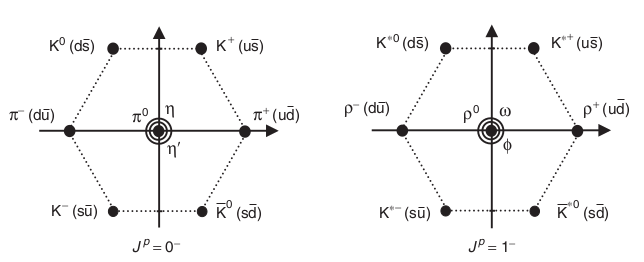
\includegraphics[width=0.6\textwidth]{mesons}
\caption{\label{trailer}\emph{All Mesons, graphed by Isospin and Hyper-charge}}
\end{figure} 
\item In terms of the quarks these are for spin-$0$:
\begin{align*}
    &\text{Pions:} 
    &|\pi^+\rangle = |u\bar{d}\rangle, \quad 
    |\pi^0\rangle = \frac{1}{\sqrt{2}} (|u\bar{u}\rangle - |d\bar{d}\rangle), \quad
    |\pi^-\rangle = |d\bar{u}\rangle \\[5pt]
    &\text{Kaons:} 
    &|K^+\rangle = |u\bar{s}\rangle, \quad
    |K^0\rangle = |d\bar{s}\rangle, \quad
    |\bar{K}^0\rangle = |s\bar{d}\rangle, \quad
    |K^-\rangle = |s\bar{u}\rangle \\[5pt]
    &\text{Eta and Eta Prime:} 
    &|\eta\rangle = \frac{1}{\sqrt{6}} (|u\bar{u}\rangle + |d\bar{d}\rangle - 2|s\bar{s}\rangle), \quad
    |\eta'\rangle = \frac{1}{\sqrt{3}} (|u\bar{u}\rangle + |d\bar{d}\rangle + |s\bar{s}\rangle)
\end{align*}
\item And for the spin-$1$ mesons:
\begin{align*}
    &\text{Rho Mesons:} 
    &|\rho^+\rangle = |u\bar{d}\rangle, \quad 
    |\rho^0\rangle = \frac{1}{\sqrt{2}} (|u\bar{u}\rangle - |d\bar{d}\rangle), \quad
    |\rho^-\rangle = |d\bar{u}\rangle \\[5pt]
    &\text{Kaon* Mesons:} 
    &|K^{*+}\rangle = |u\bar{s}\rangle, \quad
    |K^{*0}\rangle = |d\bar{s}\rangle, \quad
    |\bar{K}^{*0}\rangle = |s\bar{d}\rangle, \quad
    |K^{*-}\rangle = |s\bar{u}\rangle \\[5pt]
    &\text{Omega and Phi Mesons:} 
    &|\omega\rangle = \frac{1}{\sqrt{2}} (|u\bar{u}\rangle + |d\bar{d}\rangle), \quad
    |\phi\rangle = |s\bar{s}\rangle
\end{align*}
\item The Heavy Mesons are constructed from the bottom and charm quarks in a similar way. 
\end{itemize}
% subsection light_mesons (end)

\subsection{Baryons} % (fold)
\label{sub:baryons}
\begin{itemize}
    \item Baryons are combinations of $3$ quarks/ anti-quarks. This makes them fermions of spin $\frac{1}{2}$ or $3/2$. This means we need to calculate $3 \otimes 3 \otimes 3$. It turns out that the calculation of $3 \otimes 3$ is a little different to that of $3 \otimes \bar{3}$. Since we dont have anti-quarks we can't properly form a state that has $I_3=Y_3 =0$. This means the decomposition is $3 \otimes 3 = 6 \oplus 3$. This can be prooved by the standard ladder operator calculations. We are then left with $3 \otimes \left(6 \oplus 3\right)$ which breaks down into the standard $3 \otimes \bar{3} = 8 \oplus 1$ and the new $3 \otimes 6 = 10 \oplus 8$. Overall this means the full decomposition is:
\begin{flalign*}
    3 \otimes 3 \otimes 3 = 10 \oplus 8 \oplus 8 \oplus 1
\end{flalign*}
\item We can visulze this nicely with the followong:
    \begin{figure}[H]
\centering
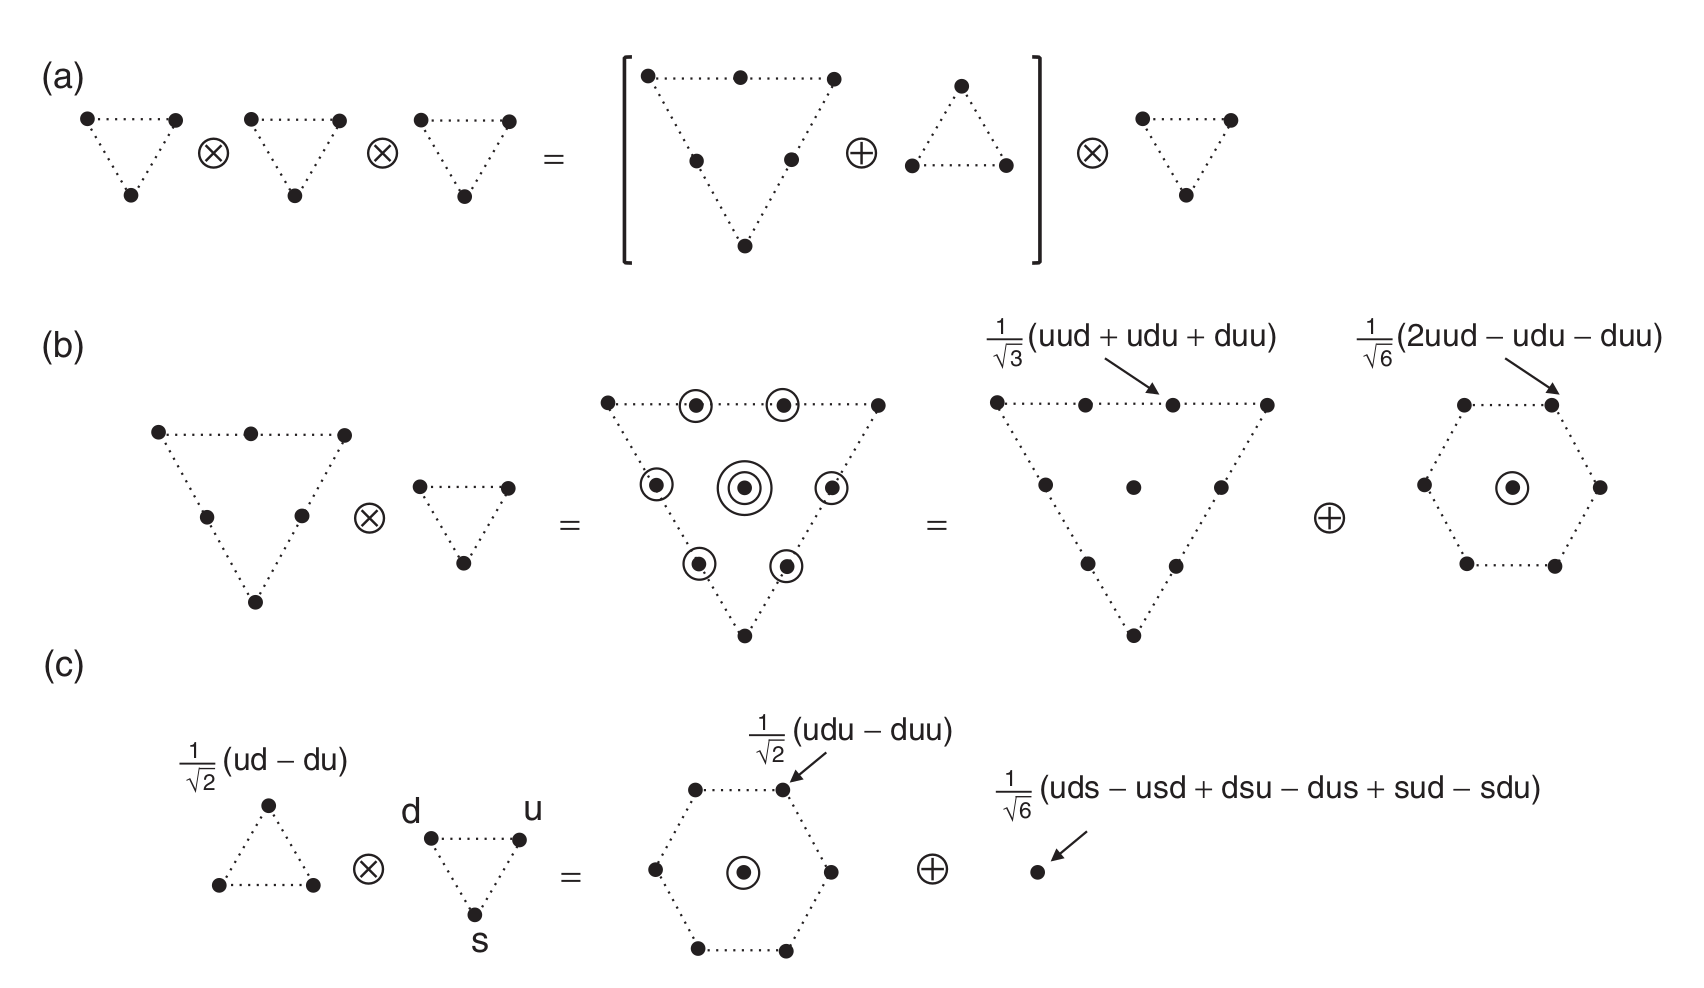
\includegraphics[width=0.8\textwidth]{3x3x3}
\caption{\label{trailer}\emph{All Mesons, graphed by Isospin and Hyper-charge}}
\end{figure}
\item The quark composition of the individual Baryons is then:
\begin{align*}
    &\text{Nucleons:} 
    &|p\rangle = |uud\rangle, \quad 
    |n\rangle = |udd\rangle \\[5pt]
    &\text{Delta Baryons:} 
    &|\Delta^{++}\rangle = |uuu\rangle, \quad
    |\Delta^+\rangle = |uud\rangle, \quad
    |\Delta^0\rangle = |udd\rangle, \quad
    |\Delta^-\rangle = |ddd\rangle \\[5pt]
    &\text{Sigma Baryons:} 
    &|\Sigma^+\rangle = |uus\rangle, \quad
    |\Sigma^0\rangle = |uds\rangle, \quad
    |\Sigma^-\rangle = |dds\rangle \\[5pt]
    &\text{Xi Baryons:} 
    &|\Xi^0\rangle = |uss\rangle, \quad
    |\Xi^-\rangle = |dss\rangle \\[5pt]
    &\text{Omega Baryon:} 
    &|\Omega^-\rangle = |sss\rangle
\end{align*}
\end{itemize}
% subsection baryons (end)
\subsection{Total Wavefunction} % (fold)
\label{sub:total_wavefunction}
\begin{itemize}
    \item There are many possible values of flavour, spin and colour (which we will encounter later) that a Baryon can have:
    \begin{align*}
        \psi = \phi_{\text{flavour}}\chi_{\text{spin}}\xi_{\text{colour}}\eta_{\text{space}}
    \end{align*}
    However, not all of these states are valid as since baryons are fermions, there total wave-functions needs to be anti-symmetric under exchange of any two quarks. We will see later that the colour wavefunction $\xi_{\text{colour}}$ is totally anti-symmetric. We are discussing the quarks with $l=0$, so zero spatial angular momentum , and since the spatial wavefunction transforms by $(-1)^l$ under parity, then $\eta_{\text{space}}$ is symmetric. This means that $ \phi_{\text{flavour}}\chi_{\text{spin}}$ must be symmetric. This allows us to determine the wave-function super positions of the quarks in terms of their flavour and spin. 
\end{itemize}
% subsection total_wavefunction (end)



\newpage
\section{Scattering \& Decay} % (fold)
\label{sec:scattering}
\begin{itemize}
    \item We will need to develop some mathematical tools for studying scattering of particles and Decay.
\end{itemize}

\subsection{Decay} % (fold)
 \label{sub:decay}
 \begin{itemize}
     \item Unstable particles have an equal probability of decaying at every instant in time. This means the probability of survival to time $t$ for a particle A is governed by:
     \begin{align*}
         &\frac{dP}{dt} = -\Gamma_A P \\
         \implies & P \propto e^{-\Gamma_At}
     \end{align*}
     The constant $\Gamma_A$ is known as the \emph{total width}. If there are multiple decay processes $A \rightarrow f$, then the total width is $\Gamma_A = \sum_f\Gamma(A \rightarrow f)$. The probability ratio of the decay into an individual particle $f$ is known as the \emph{branching ratio}: 
     \begin{align*}
         BR(A \rightarrow f) = \frac{\Gamma(A\rightarrow f)}{\Gamma_A} 
     \end{align*}
 \end{itemize}
 % subsection decay (end) 

 \subsection{Cross Section} % (fold)
 \label{sub:cross_section}
 \begin{itemize}
     \item The main object to interest to us in calculations will be the cross section, as this is measurable. Our scattering setup to calculate the cross section will be as follows. We consider a beam of A particles of density $n_A$ at a velocity $v_A$ at a target B:
\begin{figure}[H]
\centering
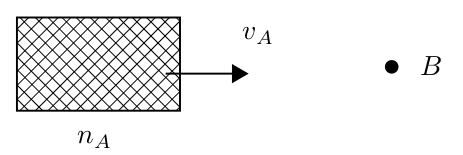
\includegraphics[width=0.6\textwidth]{scatter}
\caption{\label{trailer}\emph{Scattering setup}}
\end{figure}
\item The rate of scattering is then given by:
\begin{align*}
    \frac{\text{events}}{\text{sec}} = n_Av_A\sigma
\end{align*}
Where $\sigma$ is the cross section. It is useful for our calculations to consider all possible momenta the $n$ particles created in the process could have. The probability of finding each given momentum configuration of the final particles is given by the \emph{differential cross section}: $d\sigma/(d^3p_1 \cdot \cdot \cdot d^3p_n)$, which is related to the cross section by:
\begin{align*}
    \sigma = \int d^3p_1 \cdot \cdot \cdot d^3p_n\frac{d\sigma}{d^3p_1 \cdot \cdot \cdot d^3p_n}
\end{align*}

 \end{itemize}
 % subsection cross_section (end)

 \subsection{Master Formula} % (fold)
 \label{sub:master_formula}
 \begin{itemize}
     \item We know from our study of Quantum Field Theory \footnote{See my notes on QFT \href{https://tbrosnan12.github.io/documents/Fourth_year/First_semester/Quantum_Field_Theory_I.pdf}{here}.}, that the quantum mechanical transition matrix element is given by:
     \begin{align*}
         \bra{12 \cdot \cdot \cdot n}T \ket{A(p_A)} = \mathcal{M}(A \rightarrow 1 +2 + \cdot \cdot \cdot n)(2\pi)^4\delta(p_A - \sum_jp_j)
     \end{align*}
     Where $T$ is the time evolution operator. The factor of $\mathcal{M}$ is called the \emph{invariant Matrix element}. 
     \item To find the total rate of decay we need to integrate over the total phase, i.e. all momenta that the particles could have subject to the constraint of momentum conservation. This will be written as:
     \begin{align*}
          \int d\Pi_n = \int \frac{d^3p_1}{(2\pi)^32E_1} \cdot \cdot \cdot \frac{d^3p_n}{(2\pi)^32E_n}(2\pi)^4\delta(p_A - \sum_jp_j)
      \end{align*} 
Where we also for convenience have included in this the factors of $1/2E$, so as to satisfy Lorentz invariance.
\item Another formula we will then need from QFT is a version of Fermi's Golden rule, which tells us the particle width for a given transition to an $n-$particle final state $f$:
\begin{align*}
    \Gamma(A \rightarrow f) = \frac{1}{2m_A}\int d\Pi_n|\mathcal{M}(A\rightarrow f)|^2
\end{align*}
If the final products have spin we will need to sum over these spins. Similarly we need to do the same for the initial state, but often this state is unknown so we simply average over all possible spins instead. This expression is actually a simplification of the following more general expression for the cross section in therms of the invariant matrix element:
\begin{align*}
    \sigma(A+B \rightarrow f) = \frac{1}{2E_A2E_B|v_A-v_B|}\int d\Pi_n|\mathcal{M}(A\rightarrow f)|^2
\end{align*}

 \end{itemize}
 % subsection master_formula (end)

 \subsection{2 Particle Collision} % (fold)
 \label{sub:2_particle_collision}
 \begin{itemize}
     \item We can now use the above equations to analyze the problem of a two particle collision. We will impotently do this for the case where $\mathcal{M}$ is constant, as this represents the case where each point in the phase space is equally likely. We will consider an initial state of momentum $P$ and a final state of two particles with momentum $\textbf{p}_1$ and $\textbf{p}_2$.In this scenario the phase space integral is just:
     \begin{align}
     \label{2_phase}
         \int \Pi_2 = \int \frac{d^3p_1}{(2\pi)^32E_1}\frac{d^3p_2}{(2\pi)^32E_2}(2\pi)^4\delta^{(4)}(P-p_1-p_2)
     \end{align}
 If we work in Center of Mass (CoM) frame, where $\textbf{P}=0$, then the three spatial parts of the delta function enforce that: $\textbf{p}_1=-\textbf{p}_2$ and thus if $P = (E_{\text{CM}},0) \implies p_1=(E_1,\textbf{p}) \& p_2=(E_2,-\textbf{p})$, where the particles are on shell so $E_1 = \sqrt{p^2+m_1^2}$ and $E_2 = \sqrt{p^2+m_2^2}$. With this \ref{2_phase} becomes:
     \begin{align}
     \label{2_phase_2}
         \int \Pi_2 = \int \frac{d^3p}{(2\pi)^3}\frac{2\pi}{2E_12E_2}\delta(E_{\text{CM}}-E_1-E_2)
     \end{align}
     In spherical co-ords this volume element is just $d^3p=p^2dpd\Omega$. We can then deal with this integral by using the property of the delta function for a function with only one zero at $x_0$:
     \begin{align*}
         &\delta(f(x)) = \frac{1}{|f'(x_0)|}\delta(x-x_0) \\
         \implies  & \delta(E_{\text{CM}}-E_1(p)-E_2(p)) = \frac{\delta(p-\tilde{p})}{|dE_1/dp+dE_2/dp|}
     \end{align*}
         We can evaluate from the on-shell conditions that $dE_1/dp = p/E_1$ and $dE_2/dp = p/E_2$, so we can write \ref{2_phase_2} as:
     \begin{align*}
          \int \Pi_2 &= \int \frac{\tilde{p}^2d\Omega}{16\pi^2E_1E_2}\frac{1}{|\tilde{p}/E_1+\tilde{p}/E_2|} = \frac{1}{E_1+E_2}\int \frac{\tilde{p}d\Omega}{16\pi^2} 
     \end{align*}
     \begin{flalign}
     \label{phase_2}
         = \frac{1}{8\pi}\left(\frac{2\tilde{p}}{E_{\text{CM}}}\right)\int\frac{d\Omega}{4\pi} 
     \end{flalign}
     We can note that in the relativistic limit $E>>m_1,m_2 \implies E_{\text{CM}} = E_1+E_2 \approx \tilde{p}+\tilde{p} =2\tilde{p}$, which makes the factor in brackets in \ref{phase_2} unity. This means \ref{phase_2} becomes constant in the relativistic limit. 
 \end{itemize}
 % subsection 2_particle_collision (end)
% section scattering (end)
\end{document}
    